%%%%%%%%%%%%%%%%%%%%%%%%%%%%%%%%%%%%%%%%%%%%%%%%%%%%%%%%%%%%%%%%%%%%%%%%%%%%%%%%
%%%%%%%%%%%%%%%%%%%%%%%%%%%%%%%%%%%%%%%%%%%%%%%%%%%%%%%%%%%%%%%%%%%%%%%%%%%%%%%%
%%%%%%%%%%%%%%%%%%%%%%%%%%%%%%%%%%%%%%%%%%%%%%%%%%%%%%%%%%%%%%%%%%%%%%%%%%%%%%%%
\section{Regressão}

\index{Regressão}

\begin{wrapfigure}{l}{0.5\textwidth}
     \centering
     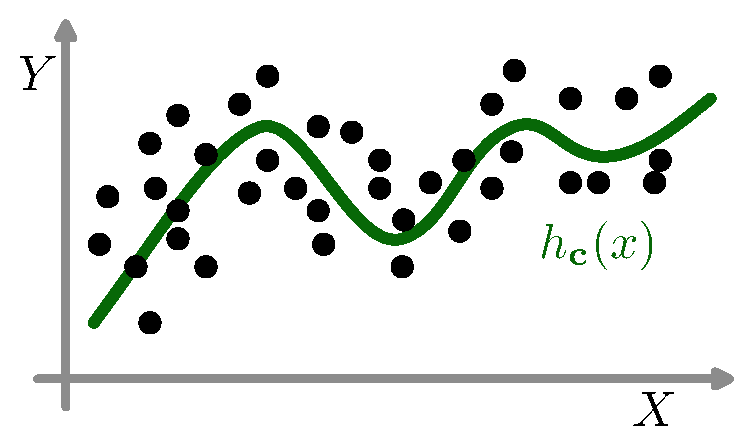
\includegraphics[width=0.45\textwidth]{chapters/notacao/regressao1.eps}
     \caption{Regressão de uma curva $h_{\VECTOR{c}}(x)$ com parâmetros $\VECTOR{c}$ num conjunto de dados. }
     \label{fig:regressao:1}
    \hspace{20pt}
\end{wrapfigure}
A regressão é o processo pelo qual uma curva ou superfície em múltiplas dimensões é 
ajustada num conjunto de dados, quando se sabe ou se aceita que existirá um erro no ajuste
devido à natureza ruidosa dos dados \cite[pp. 5]{chapra2016metodos}.

A ideia geral da regressão é achar uma curva de ajuste que represente melhor 
aos dados, sem que a curva necessariamente coincida de forma exata com todos eles,
pelo que devemos definir algum critério de medida do erro de ajuste 
e procurar uma curva que minimize este erro \cite[pp. 7]{chapra2016metodos}.

Assim, a regressão pode ser classificada mediante o tipo de curva de ajuste que é proposta;
nesse sentido podemos ver na literatura:

\begin{itemize}
\item \textbf{Regressão linear}: 
Este caso acontece quando usamos uma linha reta;
é dizer uma função $h_{\VECTOR{c}}:\mathbb{R} \rightarrow \mathbb{R}$ de parâmetros $\VECTOR{c}$, 
para aproximar um conjunto de dados \cite[pp. 398, 402]{chapra2016metodos} \cite[pp. 25]{aster2013parameter}.
A regressão linear é um caso particular da regressão polinomial quando $M=1$.
\begin{example}~
\begin{itemize}
\item Curva de ajuste na regressão linear, 
\begin{equation}
h_{\VECTOR{c}}(x)=c_1+c_2 x.
\end{equation}
\item Na Seção \ref{sec:theo:reglogr1r1:1} apos uma linearização de uma relação não linear,
como na função logística, podemos ver exemplos de regressão linear.
\end{itemize}
\end{example}

\item \textbf{Regressão polinomial}: 
Indica que usamos um polinômio de grau $M$,
representado com uma função $h_{\VECTOR{c}}:\mathbb{R} \rightarrow \mathbb{R}$ com parâmetros $\VECTOR{c}$, 
 para aproximar um conjunto de dados \cite[pp. 399, 415]{chapra2016metodos}.
\begin{example}~
\begin{itemize}
\item Um caso de curva de ajuste na regressão polinomial com grau $M=2$,
\begin{equation}
h_{\VECTOR{c}}(x)=c_1+c_2 x+c_3 x^2.
\end{equation}
\item Na Seção \ref{sec:theo:maphxr1r1} podemos ver exemplos de regressão polinomial.
\item Na Seção \ref{sec:theo:reglogr1r1poly:1} apos uma linearização de uma relação não linear,
como na função logística, podemos ver exemplos de regressão polinomial.
\end{itemize}
\end{example}

\item \textbf{Regressão não linear}: 
Neste caso usamos um ajuste de dados
com uma função $h_{\VECTOR{c}}:\mathbb{R} \rightarrow \mathbb{R}$ com parâmetros $\VECTOR{c}$, 
que representa uma relação não linear entre o domínio e o contradomínio de $h_{\VECTOR{c}}$ 
\cite[pp. 424]{chapra2016metodos} \cite[pp. 217]{agarwal2014creators}.
\begin{example}~
\begin{itemize}
\item Um caso de curva de ajuste na regressão não linear, 
\begin{equation}
h_{\VECTOR{c}}(x)=c_1 e^{-c_2 x}
\end{equation}
\item Na Seção \ref{sec:theo:maphcxr1r1} podemos ver exemplos de regressão não lineal.
\end{itemize}
\end{example}

\item \textbf{Regressão linear múltipla}:
Temos este caso quando ajustamos um hiperplano;
é dizer usamos uma função $h_{\VECTOR{c}}:\mathbb{R}^{N} \rightarrow \mathbb{R}$ com parâmetros $\VECTOR{c}$, 
para aproximar um conjunto de dados \cite[pp. 399, 418]{chapra2016metodos}.
A regressão linear é um caso particular da regressão linear múltipla quando $N=1$.
\begin{example}~
\begin{itemize}
\item Curva de ajuste na regressão linear múltipla com $N=2$, 
\begin{equation}
h_{\VECTOR{c}}(\VECTOR{x})=c_1+c_2 x_1+c_3 x_2.
\end{equation}
\item Na Seção \ref{sec:theo:reglogrnr1:1} apos uma linearização de uma relação não linear,
como na função logística, podemos ver exemplos de regressão linear múltipla.
\end{itemize}
\end{example}

\item \textbf{Regressão polinomial múltipla}:
Acontece quando ajustamos um polinômio multivariado de grau total $M$,
é dizer usamos uma função $h_{\VECTOR{c}}:\mathbb{R}^{N} \rightarrow \mathbb{R}$ com parâmetros $\VECTOR{c}$, 
para aproximar um conjunto de dados.
A regressão polinomial é um caso particular da regressão polinomial múltipla quando $N=1$.
\begin{example}~
\begin{itemize}
\item Um caso de curva de ajuste na regressão polinomial múltipla com $N=2$ e $h_{\VECTOR{c}}:\mathbb{R}^{2} \rightarrow \mathbb{R}$, 
\begin{equation}
h_{\VECTOR{c}}(\VECTOR{x})=c_1+c_2 x_1+c_3 x_2+c_4 x_1^2+c_5 x_2^2+c_6 x_1 x_2.
\end{equation}
\item Nas Seções \ref{sec:theo:maphxr2r1} e \ref{sec:theo:maphxr2r2} podemos ver exemplos de regressão polinomial múltipla.
\item Na Seção \ref{sec:theo:reglogrnr1poly:1} apos uma linearização de uma relação não linear,
como na função logística, podemos ver exemplos de regressão polinomial múltipla.
\end{itemize}
\end{example}

\item \textbf{Regressão não linear múltipla}: 
Estamos neste caso quado usamos no ajuste dos dados
uma função $h:\mathbb{R}^{N} \rightarrow \mathbb{R}$ 
que representa uma função não linear entre o domínio e o contradomínio de $h$.
A regressão não linear é um caso particular da regressão não linear múltipla quando $N=1$.
\begin{example}~
\begin{itemize}
\item Um caso de curva de ajuste na regressão não linear múltipla, 
\begin{equation}
h_{\VECTOR{c}}(\VECTOR{x})=c_1 e^{- c_2^2(x_1 -c_3)^2- c_4^2(x_1 -c_5)^2}
\end{equation}
\item Na Seção \ref{sec:theo:maphcxrnr1} podemos ver exemplos de regressão não lineal múltipla.
\item Na Seção \ref{sec:theo:reglogrnr1nolinear:1} apos uma linearização de uma relação não linear,
como na função logística, podemos ver exemplos de regressão não linear múltipla.
\end{itemize}
\end{example}
\end{itemize}
